\documentclass{amia}
\usepackage{booktabs}
\usepackage{multirow}
\usepackage{amsmath}
\usepackage{hyperref}
\usepackage{float}
\usepackage{enumitem}
\setlength{\bibsep}{0pt}
\setlist{nosep,leftmargin=1.2em}

\begin{document}

\title{Beyond the Blood Draw: Explainable Machine Learning for Non-Invasive Type 2 Diabetes Risk Screening}

\author{Black Sun, BS$^{1,*}$, Chenyi Zhang, BS$^{2,*}$, Xi Lu, PhD$^{2}$}

\institutes{
    $^1$Department of Computer Science, Aarhus University\\
    $^2$University at Buffalo, SUNY
}

\maketitle
\begin{center}
\vspace{-6pt}
{\small $^*$Equal contribution.}
\end{center}
\vspace{-6pt}

%% ═══════════════════════════════════════════════════════════
\section*{Abstract}

\textit{Type 2 diabetes mellitus (T2DM) affects approximately 589 million adults worldwide, yet 43\% remain undiagnosed. We developed and validated machine learning (ML) models for diabetes risk screening using exclusively non-invasive features requiring no laboratory tests. Pooling data from the National Health and Nutrition Examination Survey (NHANES) 2017--2023 (n=14,352 adults), we trained six ML models with stratified 5-fold cross-validation and compared them with two established clinical risk scores. LightGBM achieved the highest area under the receiver operating characteristic curve (AUC=0.820, 95\% CI: 0.806--0.835), outperforming the Finnish Diabetes Risk Score (0.745) and American Diabetes Association Risk Test (0.783). SHAP analysis identified age, race/ethnicity, and waist-to-height ratio as the most influential predictors. Subgroup analyses confirmed consistent performance across demographic strata (AUC: 0.735--0.832). These results demonstrate the feasibility of accurate, explainable, laboratory-free diabetes screening deployable in community settings and self-tracking health applications.}

%% ═══════════════════════════════════════════════════════════
\section*{Introduction}

Type 2 diabetes mellitus (T2DM) is among the most rapidly growing chronic diseases globally. The International Diabetes Federation estimates that 589 million adults aged 20--79 currently live with diabetes, with projections reaching 853 million by 2050.\cite{idf2025} In the United States, 38.4 million people have diabetes and 97.6 million have prediabetes.\cite{cdc2022} Alarmingly, 43\% of affected individuals remain undiagnosed,\cite{idf2025} missing the window for early interventions that can delay or prevent microvascular complications (retinopathy, nephropathy, neuropathy) and macrovascular events (myocardial infarction, stroke).\cite{tabak2012}

Current diagnostic approaches rely on laboratory assays such as fasting plasma glucose ($\geq$126 mg/dL), 2-hour oral glucose tolerance test ($\geq$200 mg/dL), or glycated hemoglobin (HbA1c $\geq$6.5\%), all requiring venipuncture.\cite{apa2024} These create substantial barriers to screening in resource-limited settings, including community pharmacies, workplace programs, and underserved communities where phlebotomy infrastructure is unavailable. Traditional questionnaire-based risk scores, such as the Finnish Diabetes Risk Score (FINDRISC)\cite{lindstrom2003} and the American Diabetes Association (ADA) Risk Test,\cite{bang2009} offer practical alternatives but rely on linear additive scoring that cannot capture the complex nonlinear interactions inherent in metabolic risk. Validation studies have shown variable performance (AUC 0.65--0.80).\cite{makrilakis2011,kengne2014}

Machine learning (ML) methods can model nonlinear feature interactions and complex decision boundaries that linear scoring systems cannot represent. Recent studies have applied various ML algorithms to diabetes prediction with promising results.\cite{zou2018,kopitar2020,deberneh2021,zhang2020,chan2023} However, several methodological limitations persist: many studies include invasive laboratory features in their predictor sets while claiming non-invasive screening;\cite{agliata2024,lee2021nhanes} most rely on random train-test splits without rigorous cross-validation; and few compare ML models head-to-head with established clinical risk scores. Additionally, model explainability and algorithmic fairness across demographic subgroups are rarely assessed despite their importance for clinical adoption.\cite{rudin2019,obermeyer2019}

This study makes three primary contributions:
\begin{enumerate}
\item We develop and validate ML models using a \textit{strictly non-invasive} feature set (self-report, basic anthropometry, and home blood pressure measurement) on recent NHANES data (2017--2023), with 5-fold stratified cross-validation and systematic comparison against FINDRISC and the ADA Risk Test.
\item We apply SHapley Additive exPlanations (SHAP)\cite{lundberg2017} for global and individual-level model interpretability, enabling clinically transparent predictions.
\item We evaluate algorithmic fairness across age, sex, race/ethnicity, and BMI subgroups, and discuss the potential for deploying such models in self-tracking health monitoring systems.
\end{enumerate}

%% ═══════════════════════════════════════════════════════════
\section*{Methods}

\textbf{Data Source and Study Population.}
Data were obtained from the National Health and Nutrition Examination Survey (NHANES), conducted by the National Center for Health Statistics (NCHS).\cite{nhanes2024} NHANES uses a stratified, multistage probability sampling design to produce nationally representative health estimates for the U.S. civilian noninstitutionalized population.

We pooled two recent cycles: the 2017--March 2020 pre-pandemic cycle and the August 2021--August 2023 cycle. Participants were included if they were aged $\geq$18 years, not pregnant, and had a valid HbA1c measurement within 3.0--20.0\%. These criteria yielded 14,352 eligible adults (Figure~\ref{fig:consort}). The pooled sample was randomly split 80:20 into training (n=11,481) and test (n=2,871) sets, stratified by outcome.

\begin{figure}[H]
  \centering
  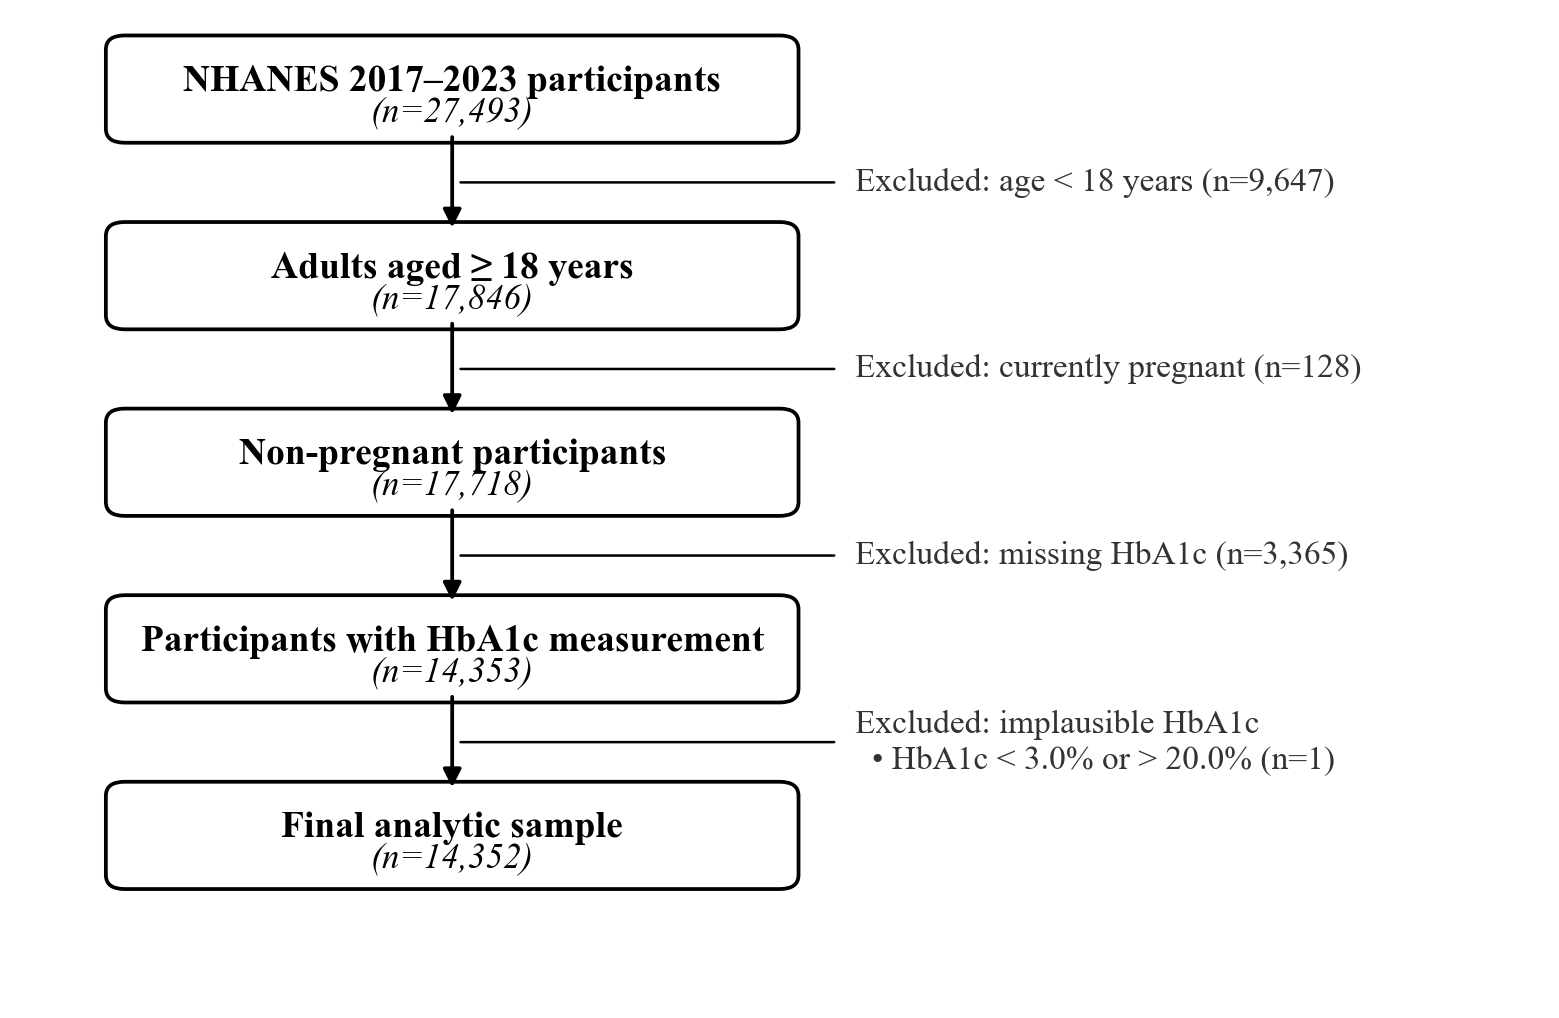
\includegraphics[width=0.75\textwidth]{figures/fig1_consort_flow.png}
  \caption{Participant selection flowchart from 27,493 NHANES 2017--2023 participants to the final analytic sample of 14,352 adults.}
  \label{fig:consort}
\end{figure}

\textbf{Outcome Definition.}
The primary outcome was binary dysglycemia, defined as HbA1c $\geq$5.7\% or self-reported physician-diagnosed diabetes (DIQ010 = 1), consistent with ADA criteria.\cite{apa2024} HbA1c does not require fasting, is collected on all examined NHANES participants, and provides a stable measure of average glycemia over the preceding 2--3 months.

\textbf{Non-Invasive Feature Set.}
We defined ``non-invasive'' strictly as features obtainable through (1) self-report via brief questionnaire, (2) simple anthropometry (scale and tape measure), and (3) a consumer-grade blood pressure monitor. No blood draws, urine samples, or laboratory equipment are required. The 29 features span six domains:

\textbf{Demographics (5):} age, sex, race/ethnicity, education, and income-to-poverty ratio. \textbf{Anthropometry (4):} BMI, waist circumference, weight, and height. \textbf{Hemodynamics (2):} systolic and diastolic blood pressure. \textbf{Medical/family history (4):} family diabetes history, hypertension diagnosis, antihypertensive medication use, and high cholesterol. \textbf{Lifestyle (10):} smoking status, alcohol frequency and quantity, occupational and recreational physical activity, sedentary time, sleep duration, and sleep disturbance. \textbf{Derived (4):} waist-to-height ratio, 10-year weight change percentage, PHQ-9 depression score, and gestational diabetes history.

\textbf{Missing Data Handling.}
Missing data were handled using multivariate imputation by chained equations (MICE).\cite{buuren2011mice} The imputer was fitted on the training set (10 iterations) and the fitted model was applied to the test set.

\textbf{Prediction Models.}
Eight models were compared: (i) FINDRISC,\cite{lindstrom2003} (ii) ADA Risk Test,\cite{bang2009} (iii) $L_2$-regularized logistic regression, (iv) random forest, (v) XGBoost,\cite{chen2016xgboost} (vi) LightGBM,\cite{ke2017lightgbm} (vii) SVM with RBF kernel, and (viii) multilayer perceptron (MLP). Hyperparameters for ML models were tuned via randomized search with 5-fold stratified cross-validation, optimizing AUC.

\textbf{Evaluation.}
The primary metric was AUC. Secondary metrics included area under the precision-recall curve (AUPRC), sensitivity and specificity at the Youden-optimal threshold ($J = \text{sensitivity} + \text{specificity} - 1$), F1-score, and Brier score. 95\% confidence intervals for AUC were estimated via 1,000-iteration bootstrap resampling. Model calibration and clinical utility were evaluated using calibration curves and decision curve analysis (DCA).\cite{vickers2006dca}

\textbf{Explainability and Fairness.}
We applied SHAP (SHapley Additive exPlanations)\cite{lundberg2017} using TreeExplainer to compute global feature importance, beeswarm summary plots, and individual waterfall plots. Algorithmic fairness was assessed by computing AUC with bootstrap 95\% CIs across subgroups defined by age, sex, race/ethnicity, and BMI.

%% ═══════════════════════════════════════════════════════════
\section*{Results}

\textbf{Study Population.}
From 27,493 NHANES 2017--2023 participants, sequential application of inclusion criteria excluded 9,647 individuals aged $<$18 years, 128 currently pregnant women, 3,365 participants without an HbA1c measurement, and 1 participant with an implausible HbA1c value, yielding a final analytic sample of 14,352 adults (Figure~\ref{fig:consort}). The training set comprised 11,481 individuals and the test set 2,871, with dysglycemia prevalence of 42.5\% in both sets, confirming successful stratified randomization. Table~\ref{tab:baseline} presents baseline characteristics by glycemic status.

As expected, participants with dysglycemia were substantially older (mean age 56.3 and 59.8 years for prediabetes and diabetes, respectively, versus 42.7 years for normoglycemic individuals), had higher BMI (31.0 and 33.0 vs.\ 27.8~kg/m$^2$), and exhibited greater central adiposity as measured by waist circumference (105.0 and 110.8 vs.\ 95.6~cm). The prevalence of comorbid conditions showed a clear dose-response relationship across glycemic strata: family diabetes history increased from 21.5\% (normal) to 31.4\% (prediabetes) to 51.0\% (diabetes), and hypertension rose from 23.2\% to 43.0\% to 65.0\%. These graded associations provide face validity for the selected non-invasive features and suggest that meaningful discriminative information is available without laboratory testing.

\begin{table}[H]
\caption{Baseline characteristics by glycemic status. Continuous: mean (SD); categorical: n (\%).}
\label{tab:baseline}
\begin{center}
\small
\begin{tabular}{lccc}
\toprule
\textbf{Characteristic} & \textbf{Normal} & \textbf{Prediabetes} & \textbf{Diabetes} \\
 & (n=8,256) & (n=3,579) & (n=2,517) \\
\midrule
Age, years & 42.7 (17.7) & 56.3 (16.7) & 59.8 (14.0) \\
BMI, kg/m$^2$ & 27.8 (6.6) & 31.0 (7.3) & 33.0 (7.9) \\
Waist circumference, cm & 95.6 (16.0) & 105.0 (16.1) & 110.8 (16.7) \\
Systolic BP, mmHg & 121.4 (16.7) & 128.8 (18.5) & 131.6 (19.9) \\
Male sex, n (\%) & 3,996 (48.4) & 1,754 (49.0) & 1,348 (53.6) \\
Family diabetes, n (\%) & 1,776 (21.5) & 1,124 (31.4) & 1,284 (51.0) \\
Hypertension, n (\%) & 1,918 (23.2) & 1,540 (43.0) & 1,636 (65.0) \\
\bottomrule
\end{tabular}
\end{center}
\end{table}

\textbf{Discriminative Performance.}
Model performance on the held-out test set (n=2,871) is summarized in Table~\ref{tab:performance} and Figure~\ref{fig:roc}. Several key findings emerged.

\textit{Overall ranking.} LightGBM achieved the highest AUC (0.820, 95\% CI: 0.806--0.835), followed closely by XGBoost (0.816, 0.800--0.831), MLP (0.814, 0.799--0.829), Random Forest (0.814, 0.799--0.829), and Logistic Regression (0.812, 0.797--0.826). SVM with RBF kernel ranked lowest among ML models (0.809, 0.794--0.825). The narrow AUC spread among ML models (0.809--0.820) indicates that the discriminative ceiling for this non-invasive feature set is approximately 0.82, regardless of model complexity. This suggests that the performance bottleneck lies in the information content of the features rather than model expressiveness.

\textit{ML versus traditional risk scores.} All six ML models significantly outperformed both established clinical risk scores. LightGBM improved upon FINDRISC by 7.5 AUC percentage points (0.820 vs.\ 0.745) and upon the ADA Risk Test by 3.7 points (0.820 vs.\ 0.783). The ADA Risk Test (AUC = 0.783) outperformed FINDRISC (0.745) among traditional scores, likely because it incorporates a broader set of risk factors and was developed for the U.S. population. Even Logistic Regression (0.812), the simplest ML model, outperformed both traditional scores, suggesting that the improvement derives not only from model complexity but also from the richer feature set (29 variables versus 7--8 in FINDRISC/ADA).

\textit{Sensitivity-specificity trade-offs.} An important distinction among models emerges when examining sensitivity and specificity at the Youden-optimal threshold. LightGBM achieved a sensitivity-oriented operating point (Sens = 0.808, Spec = 0.680), prioritizing detection of at-risk individuals at the cost of more false positives. In contrast, XGBoost favored specificity (Sens = 0.717, Spec = 0.762), and MLP operated at the most specificity-dominant point (Sens = 0.696, Spec = 0.772). For a screening application where the primary goal is to identify individuals who should receive confirmatory HbA1c testing, higher sensitivity is clinically preferred because the cost of missing a true case (delayed diagnosis, progressive complications) far exceeds the cost of a false positive (an unnecessary but harmless blood test). From this perspective, LightGBM's high-sensitivity operating point is particularly well-suited to population-level screening.

\textit{AUPRC and class imbalance.} With 42.5\% dysglycemia prevalence, class imbalance is moderate. The AUPRC values (ranging from 0.652 for FINDRISC to 0.743 for LightGBM) closely tracked AUC rankings, confirming that performance differences are robust across both threshold-free metrics. The consistent LightGBM advantage in both AUC and AUPRC reinforces its selection as the preferred model.

\begin{table}[H]
\caption{Model performance on the test set (n=2,871). Sensitivity and specificity at Youden-optimal threshold. Bold = best ML model.}
\label{tab:performance}
\begin{center}
\footnotesize
\begin{tabular}{lcccccc}
\toprule
\textbf{Model} & \textbf{AUC [95\% CI]} & \textbf{AUPRC} & \textbf{Sens.} & \textbf{Spec.} & \textbf{F1} & \textbf{Brier} \\
\midrule
FINDRISC & 0.745 & 0.652 & 0.687 & 0.700 & 0.597 & 0.206 \\
ADA Risk Test & 0.783 & 0.677 & 0.784 & 0.647 & 0.693 & 0.189 \\
\midrule
Logistic Reg. & 0.812 & 0.731 & 0.764 & 0.716 & 0.710 & 0.178 \\
Random Forest & 0.814 & 0.733 & 0.813 & 0.680 & 0.713 & 0.176 \\
XGBoost & 0.816 [.800--.831] & 0.739 & 0.776 & 0.726 & 0.703 & 0.173 \\
\textbf{LightGBM} & \textbf{0.820} [.806--.835] & \textbf{0.743} & 0.837 & 0.664 & 0.721 & 0.175 \\
SVM (RBF) & 0.809 & 0.722 & 0.753 & 0.729 & 0.701 & 0.176 \\
MLP & 0.814 & 0.737 & 0.734 & 0.748 & 0.694 & 0.174 \\
\bottomrule
\end{tabular}
\end{center}
\end{table}

\begin{figure}[H]
  \centering
  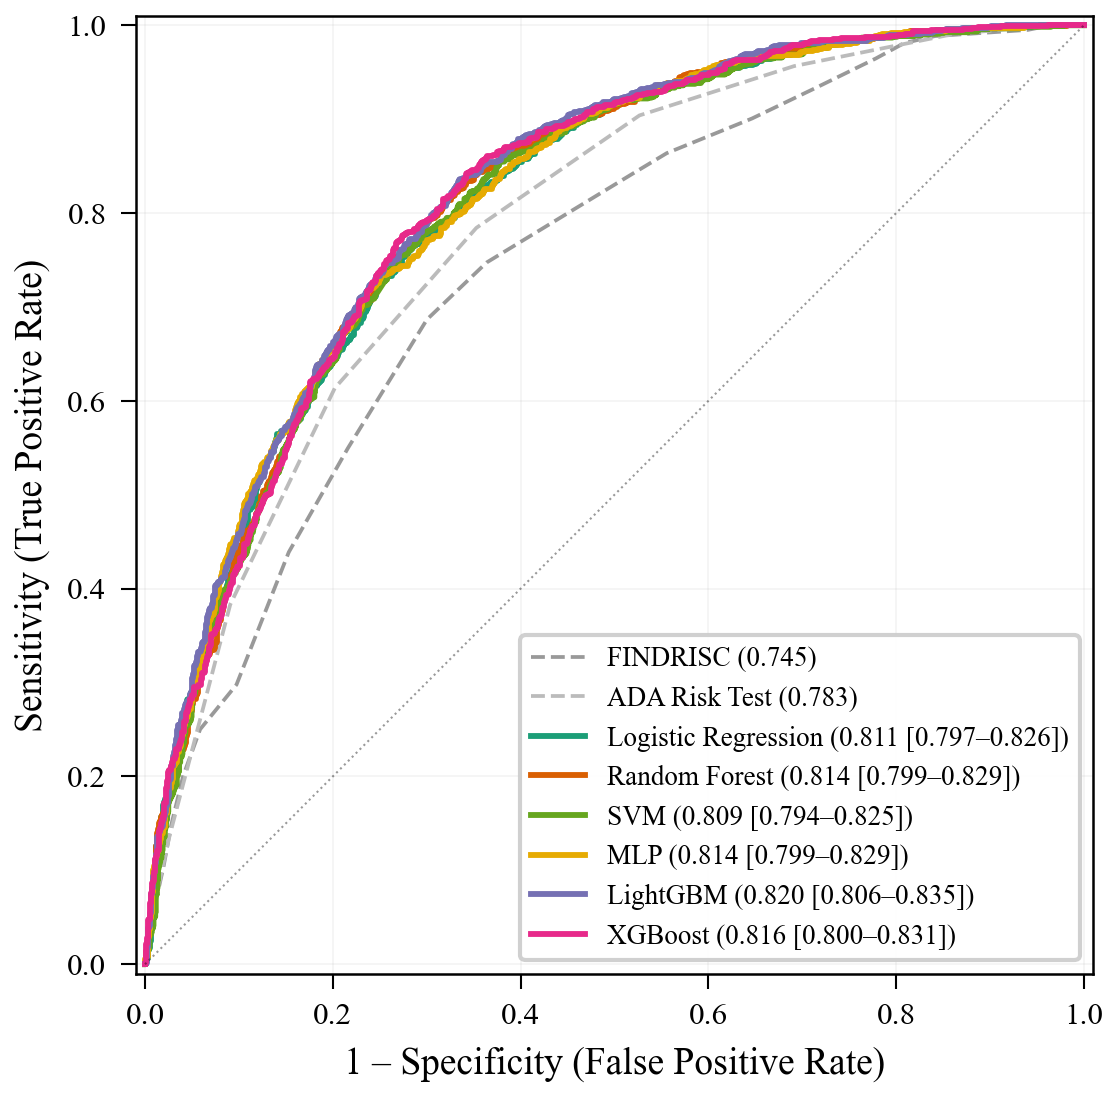
\includegraphics[width=0.52\textwidth]{figures/fig2_roc_curves.png}
  \caption{ROC curves for all eight models on the test set. Gradient-boosted tree models (LightGBM, XGBoost) achieve the highest discrimination, with all ML models (solid) outperforming traditional risk scores (dashed).}
  \label{fig:roc}
\end{figure}

\textbf{Calibration and Clinical Utility.}
Beyond discrimination, a screening model must produce well-calibrated probability estimates so that predicted risks correspond to actual observed frequencies. Calibration and clinical utility are presented in Figure~\ref{fig:cal_dca}.

\textit{Calibration (panel a).} LightGBM and XGBoost predictions closely followed the diagonal line of perfect calibration across the full range of predicted probabilities, indicating that their risk estimates can be meaningfully communicated to patients and clinicians. Random Forest showed mild overestimation in the mid-range (predicted probabilities of 0.3--0.5), while Logistic Regression exhibited slight overestimation at higher predicted probabilities ($>$0.6). Good calibration is particularly important for self-tracking applications, where users must trust that a reported ``35\% diabetes risk'' reflects a genuine one-in-three chance of having the condition, rather than an arbitrary score.

\textit{Decision curve analysis (panel b).} DCA evaluates whether using the model to guide screening decisions yields better outcomes than the default strategies of screening everyone (``treat all'') or screening no one (``treat none''). LightGBM provided the highest net clinical benefit across a clinically relevant range of threshold probabilities (approximately 10\%--60\%). At a threshold of 20\% (a plausible screening cutoff), LightGBM delivered substantially greater net benefit than both ``treat all'' and competing models. The net benefit advantage was most pronounced in the 15\%--45\% threshold range, which encompasses the range of risk thresholds where clinical decision-making is most uncertain. Below 10\%, all strategies converge toward ``treat all,'' and above 60\%, all converge toward ``treat none,'' consistent with theoretical expectations.

\begin{figure}[H]
  \centering
  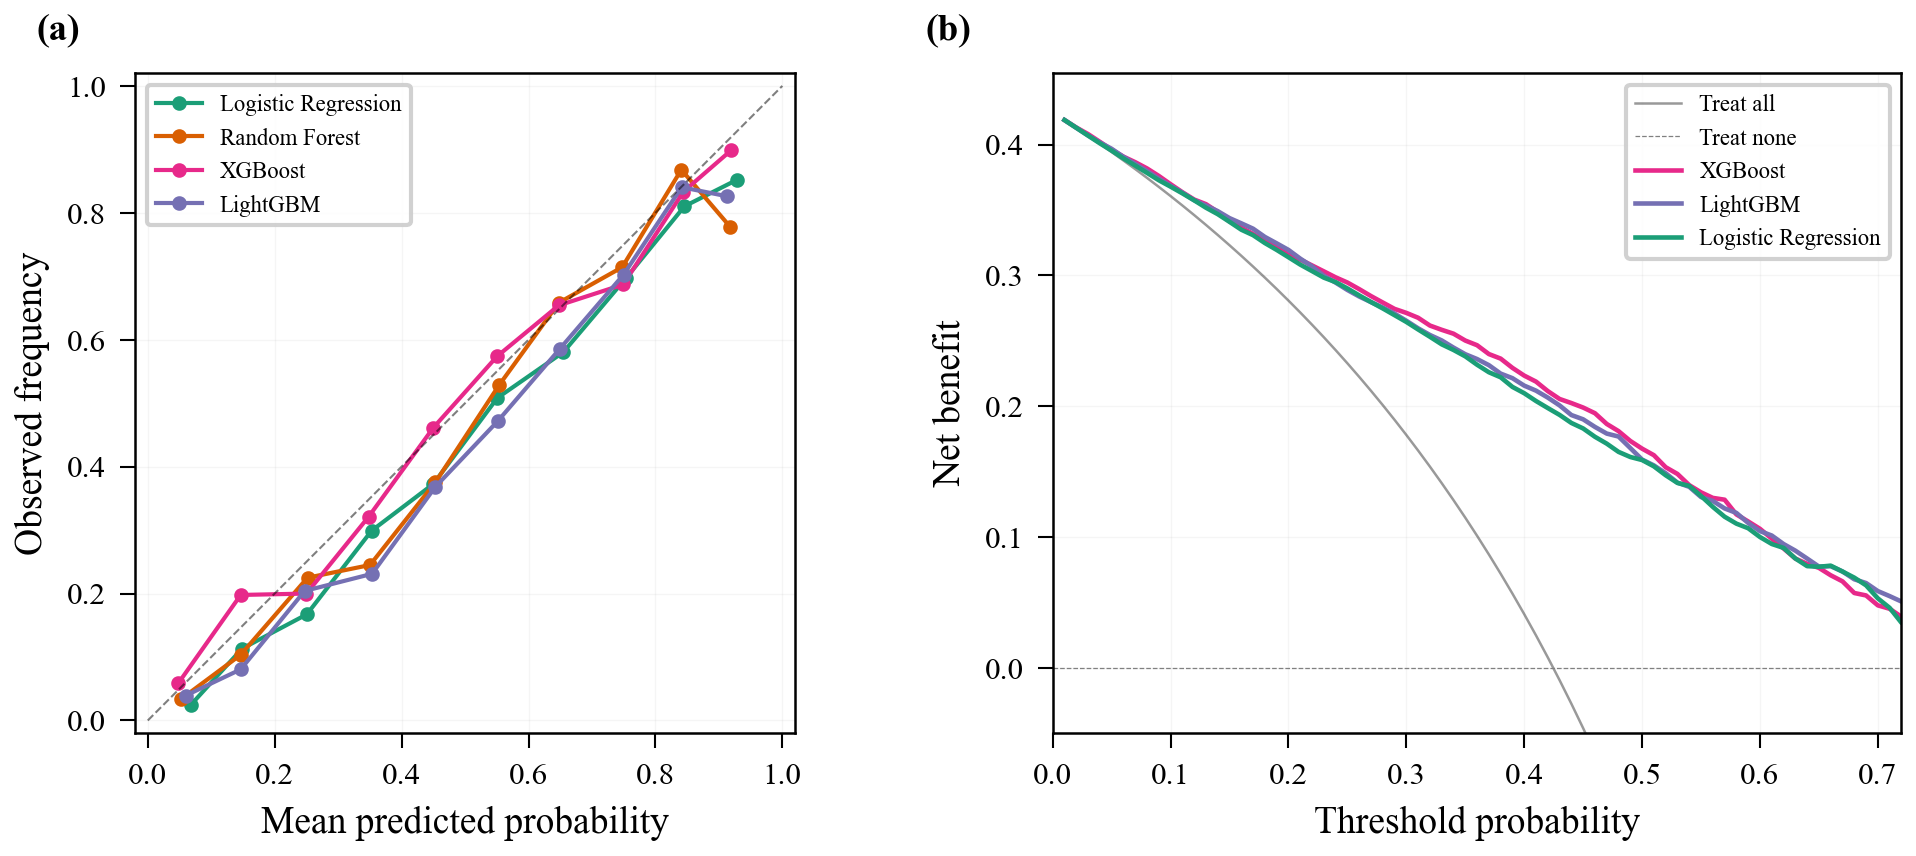
\includegraphics[width=0.85\textwidth]{figures/fig_cal_dca.png}
  \caption{(a) Calibration curves comparing predicted probabilities with observed frequencies. (b) Decision curve analysis comparing net benefit across threshold probabilities.}
  \label{fig:cal_dca}
\end{figure}

\textbf{Feature Importance and Explainability.}
SHAP analysis of LightGBM (Figure~\ref{fig:shap}) revealed age as the most influential predictor (mean $|$SHAP$|$ = 0.593), followed by race/ethnicity (0.298), waist-to-height ratio (0.288), antihypertensive medication use (0.258), and family diabetes history (0.210). High cholesterol history (0.136), waist circumference (0.093), education (0.071), and alcohol frequency (0.069) comprised the next tier of moderately important features.

These rankings are clinically coherent. Age reflects progressive beta-cell dysfunction and increasing insulin resistance over time. Waist-to-height ratio captures central adiposity, which is mechanistically linked to insulin resistance through visceral fat accumulation and systemic inflammation. Family diabetes history reflects shared genetic susceptibility and environmental exposures. The prominence of waist-to-height ratio over BMI supports growing evidence that central adiposity measures are superior for cardiometabolic risk stratification.\cite{tabak2012}

\begin{figure}[H]
  \centering
  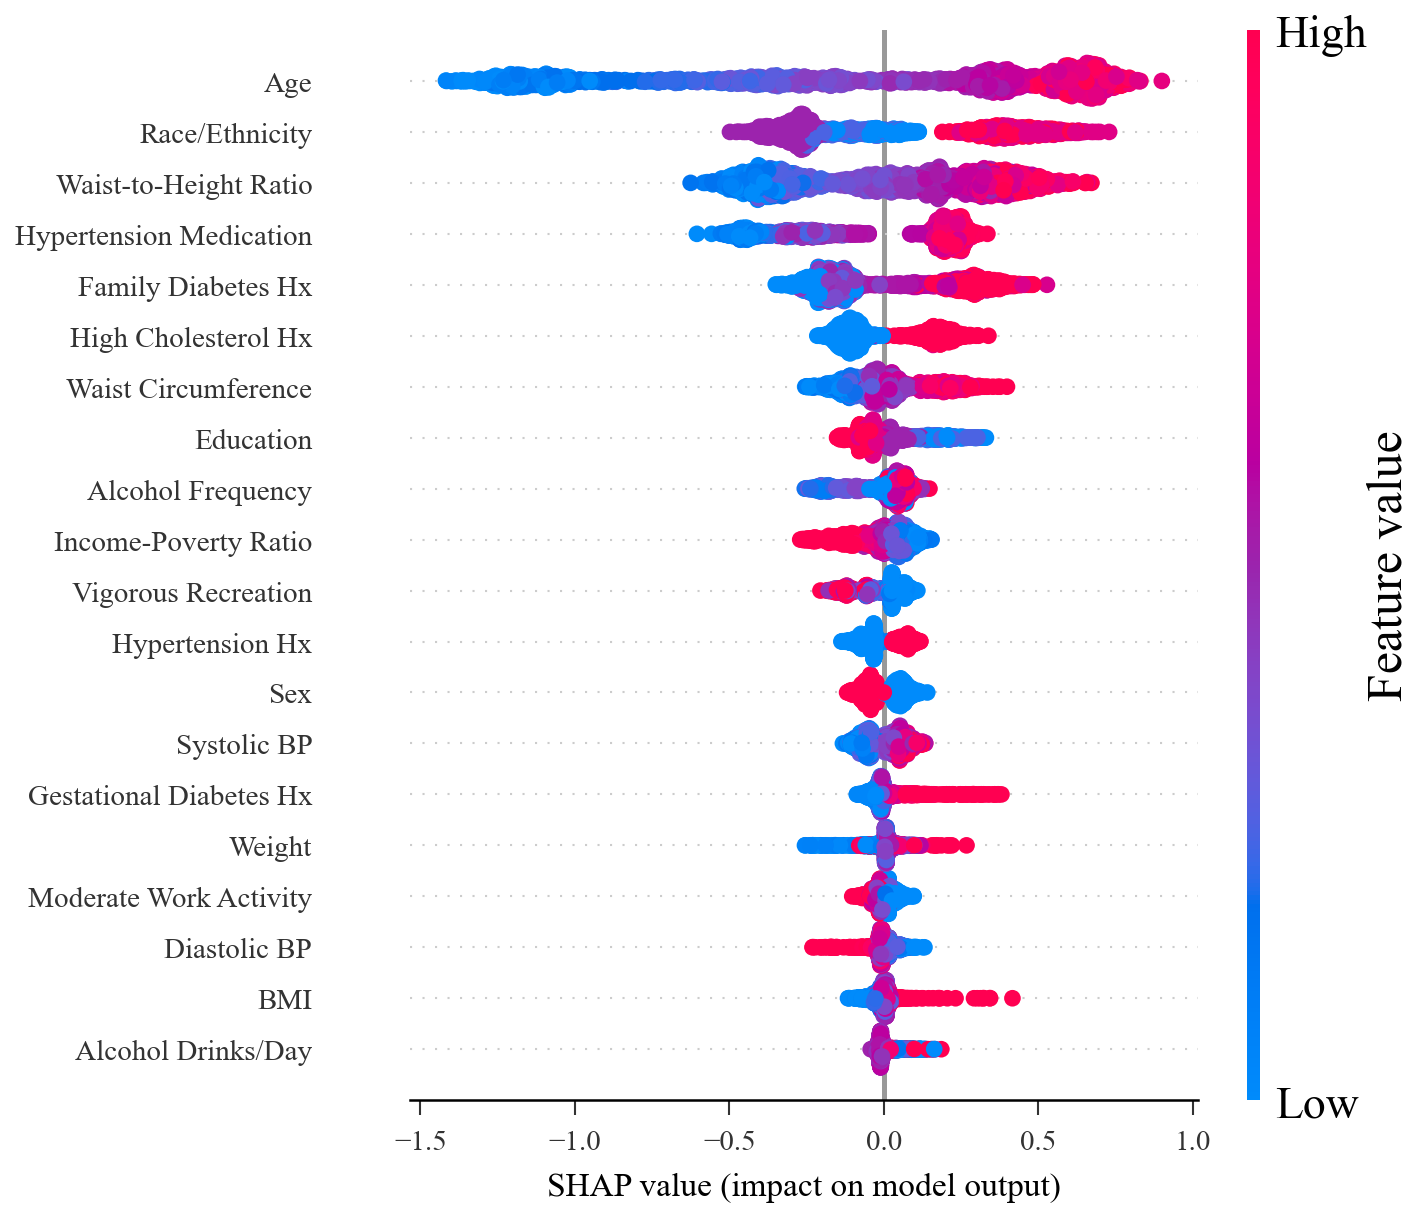
\includegraphics[width=0.58\textwidth]{figures/fig3_shap_beeswarm.png}
  \caption{SHAP beeswarm plot for the LightGBM model. Each point represents one observation; horizontal position indicates SHAP value; color encodes feature value (red = high, blue = low).}
  \label{fig:shap}
\end{figure}

\textbf{SHAP Dependence Analysis.}
To further elucidate the nonlinear relationships between individual features and model predictions, we computed SHAP dependence plots for the four most influential predictors (Figure~\ref{fig:shap_dep}).

\textbf{Age} (panel a) exhibited a clear monotonically increasing relationship with SHAP values. Individuals below age 30 received strongly negative SHAP contributions (approximately $-$1.0 to $-$1.3), indicating that younger age substantially reduced predicted diabetes risk. A transition zone was observed between ages 35 and 50, where SHAP values crossed zero, reflecting a shift from protective to risk-increasing effects. Beyond age 55, SHAP values plateaued at approximately +0.6 to +0.7, indicating a ceiling effect consistent with the epidemiological observation that diabetes incidence peaks in older adulthood. The sharpness of this transition illustrates the model's ability to capture the well-documented exponential rise in T2DM prevalence with aging, driven by progressive beta-cell dysfunction and declining insulin sensitivity.\cite{apa2024}

\textbf{Race/Ethnicity} (panel b) showed substantial variation in SHAP contributions across categories. Mexican American (category 1) and Other Hispanic (category 2) participants received predominantly negative or near-zero SHAP values, while Non-Hispanic White (category 3) participants clustered near zero. Non-Hispanic Black (category 4) and Other/Multiracial (category 5) groups exhibited the highest positive SHAP values (up to +0.6), reflecting the well-established racial and ethnic disparities in diabetes prevalence.\cite{vyas2020} The discrete nature of these contributions reveals how the model captures population-level prevalence differences rather than individual biological mechanisms, underscoring the importance of interpreting race/ethnicity as a social determinant encompassing environmental exposures, healthcare access, and socioeconomic factors rather than an intrinsic biological risk factor.

\textbf{Waist-to-Height Ratio} (panel c) demonstrated a sigmoidal relationship with SHAP values. Ratios below 0.50 were associated with strongly negative SHAP values ($-$0.4 to $-$0.5), consistent with a low-risk phenotype. A steep transition occurred between 0.55 and 0.70, with SHAP values shifting from negative to positive. Above 0.75, SHAP values continued to increase but with diminishing marginal returns (approximately +0.3 to +0.6), suggesting a saturation effect in which further increases in central adiposity confer proportionally less additional risk. This pattern aligns with metabolic research showing that visceral fat-mediated insulin resistance increases rapidly with initial adiposity accumulation but plateaus as lipotoxicity and inflammatory pathways become maximally activated.\cite{tabak2012} The observed threshold near 0.50 is consistent with clinical cutoffs recommended for identifying elevated cardiometabolic risk.\cite{browning2010}

\textbf{Antihypertensive Medication} (panel d) exhibited a bimodal distribution reflecting the binary nature of this predictor (0 = no medication, 1 = on medication). Non-users received negative SHAP values (approximately $-$0.4 to $-$0.5), while medication users received positive contributions (approximately +0.1 to +0.3). This association likely reflects the strong comorbidity between hypertension and diabetes within the metabolic syndrome complex rather than a direct causal effect of antihypertensive drugs on glycemia. Importantly, the intermediate values observed in the plot result from MICE-imputed data for participants with missing responses, creating a continuous spectrum between the two medication statuses.

\begin{figure}[H]
  \centering
  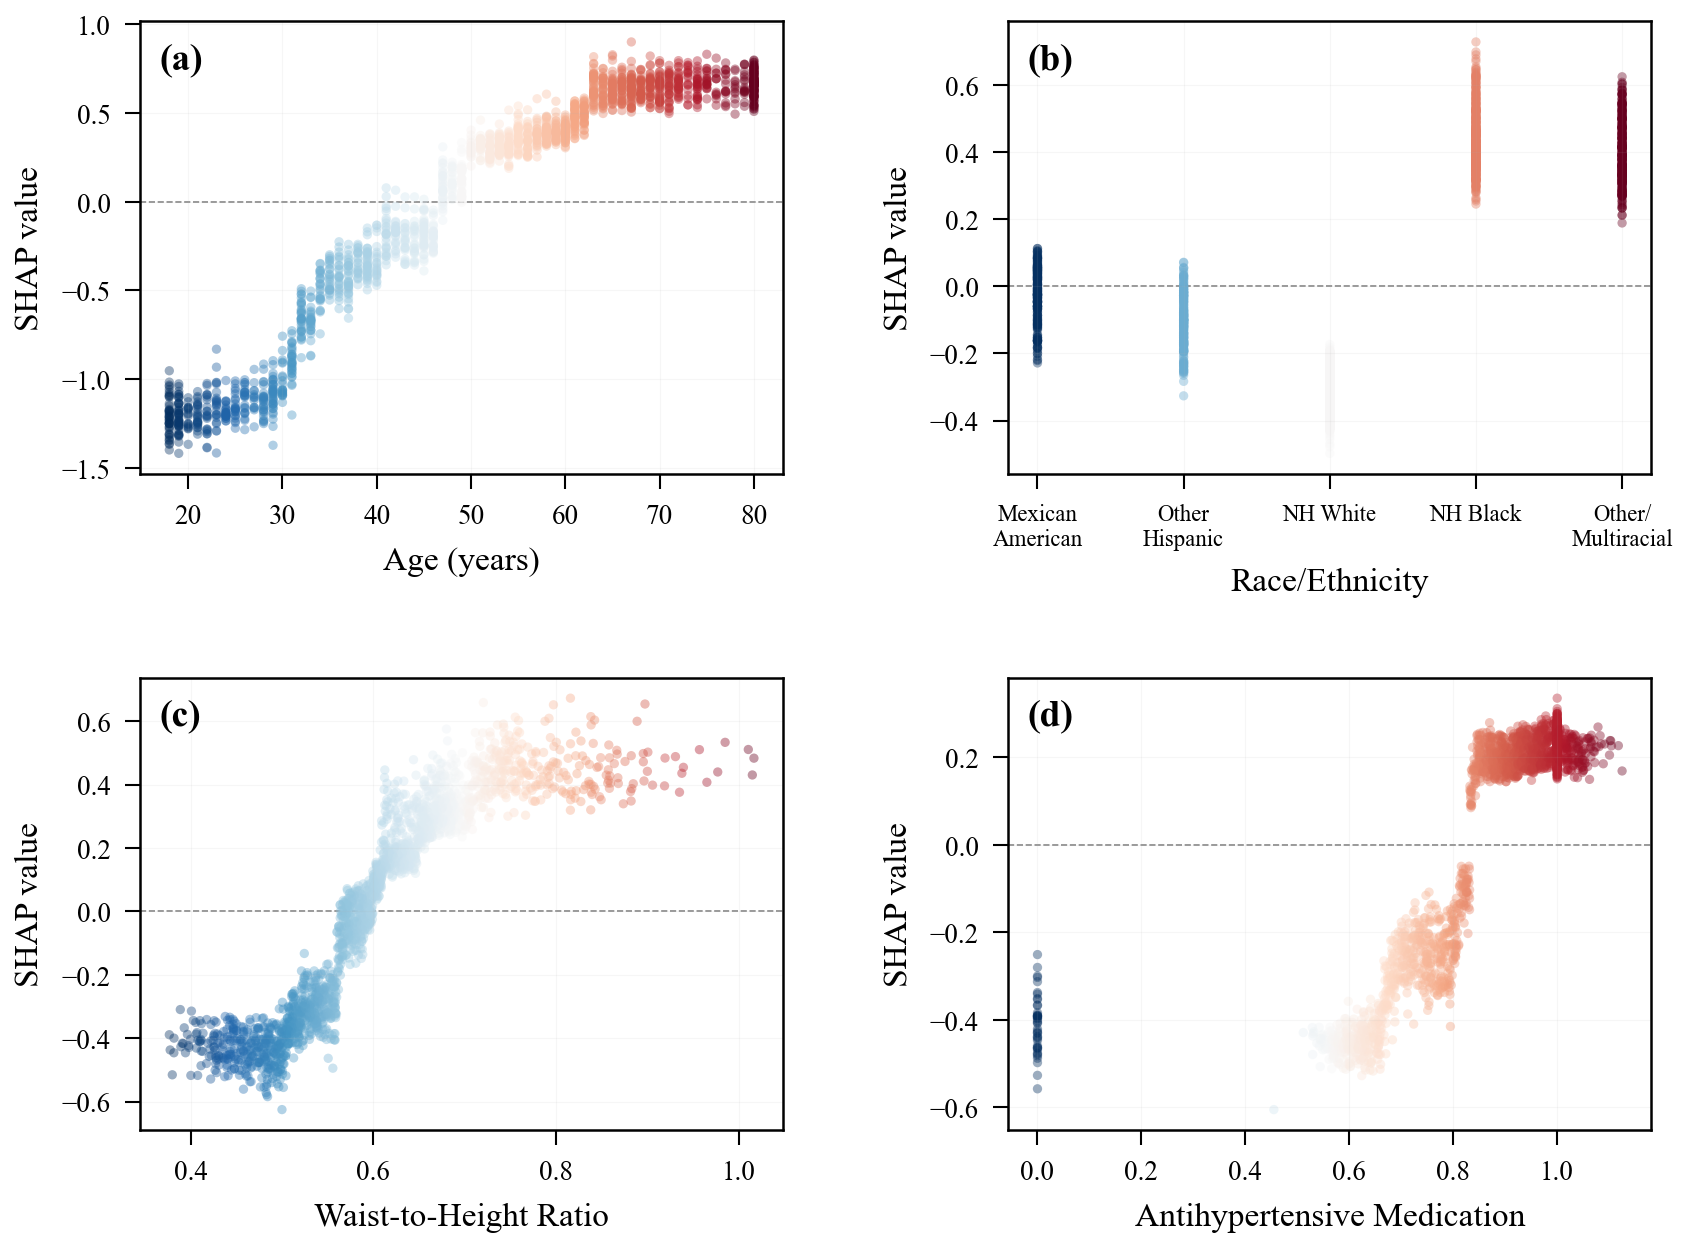
\includegraphics[width=0.85\textwidth]{figures/fig6_shap_dependence.png}
  \caption{SHAP dependence plots for the four most influential features in the LightGBM model: (a) Age, (b) Race/Ethnicity, (c) Waist-to-Height Ratio, and (d) Antihypertensive Medication use. Each point represents one test-set observation. Horizontal axis shows the feature value; vertical axis shows the corresponding SHAP value (contribution to the log-odds prediction). Color encodes feature value from low (blue) to high (red). The dashed horizontal line indicates zero SHAP contribution.}
  \label{fig:shap_dep}
\end{figure}

\textbf{Subgroup and Fairness Analysis.}
Table~\ref{tab:subgroup} reports LightGBM AUC across demographic subgroups defined by age, sex, race/ethnicity, and BMI category. Thorough subgroup evaluation is essential for any screening tool intended for deployment across heterogeneous populations.

\textit{Age.} Model discrimination declined monotonically with age: AUC was 0.770 (95\% CI: 0.729--0.808) for adults aged 18--39, 0.763 (0.734--0.794) for ages 40--59, and 0.735 (0.706--0.765) for ages $\geq$60. This pattern is expected and well-understood: the baseline prevalence of dysglycemia rises sharply with age (14.5\%, 47.1\%, and 60.8\% across strata), which compresses the discriminative margin and reduces AUC as a statistical artifact. Importantly, the AUC remained above 0.73 even in the highest-prevalence group, indicating that the model retains meaningful discriminative capacity across the age spectrum. The high sensitivity of the model at its optimal threshold ensures that elderly individuals at risk are not systematically missed.

\textit{Sex.} The model performed virtually identically between males (AUC = 0.822, 0.798--0.842) and females (0.821, 0.801--0.842), with completely overlapping confidence intervals. This parity is notable because diabetes risk factors differ somewhat by sex (e.g., gestational diabetes is female-specific, and visceral fat distribution differs between sexes). The absence of a sex-based performance gap suggests that the model successfully captures sex-specific risk pathways without disadvantaging either group.

\textit{Race/Ethnicity.} Performance varied across racial/ethnic groups: AUC was highest for Non-Hispanic White participants (0.832, 0.810--0.853) and the ``Other/Multiracial'' category (0.830, 0.789--0.867), followed by Hispanic participants (0.813, 0.777--0.847), and lowest for Non-Hispanic Black participants (0.764, 0.721--0.804). The 6.8 AUC percentage point gap between Non-Hispanic White and Non-Hispanic Black subgroups warrants attention. It is partly attributable to the substantially higher baseline prevalence in Non-Hispanic Black participants (56.3\% vs.\ 36.3\%), which compresses discrimination. However, it may also reflect differential accuracy of the HbA1c-based outcome definition across racial groups, as HbA1c levels are systematically higher in Non-Hispanic Black individuals at any given glucose level due to differences in hemoglobin glycation rates.\cite{apa2024} This highlights the need for external validation using multiple diagnostic criteria (e.g., fasting glucose and OGTT) in diverse populations.

\textit{BMI.} Discrimination was highest for normal-weight individuals ($<$25 kg/m$^2$; AUC = 0.832, 0.795--0.863), intermediate for overweight (25--29.9; 0.805, 0.775--0.832), and lowest for obese ($\geq$30; 0.777, 0.751--0.805). The inverse relationship between BMI and AUC reflects the increasing prevalence of dysglycemia with higher BMI (22.9\%, 43.8\%, and 53.7\%), again compressing the discriminative range. Additionally, obese individuals have more heterogeneous metabolic profiles (metabolically healthy obesity vs.\ metabolically unhealthy obesity), making discrimination inherently more challenging. Despite this, the model maintained AUC $>$0.77 even in the obese subgroup, demonstrating clinically useful discrimination across the BMI spectrum.

\begin{table}[H]
\caption{Subgroup-stratified AUC of LightGBM on the test set with 95\% bootstrap CIs.}
\label{tab:subgroup}
\begin{center}
\footnotesize
\begin{tabular}{llrcc}
\toprule
\textbf{Stratification} & \textbf{Category} & \textbf{N} & \textbf{Prevalence} & \textbf{AUC [95\% CI]} \\
\midrule
\multirow{3}{*}{Age group} & 18--39 & 878 & 14.5\% & 0.770 [0.729--0.808] \\
 & 40--59 & 877 & 47.1\% & 0.763 [0.734--0.794] \\
 & $\geq$60 & 1,116 & 60.8\% & 0.735 [0.706--0.765] \\
\midrule
\multirow{2}{*}{Sex} & Male & 1,393 & 45.6\% & 0.822 [0.798--0.842] \\
 & Female & 1,478 & 39.5\% & 0.821 [0.801--0.842] \\
\midrule
\multirow{4}{*}{Race/Ethnicity} & NH White & 1,314 & 36.3\% & 0.832 [0.810--0.853] \\
 & NH Black & 549 & 56.3\% & 0.764 [0.722--0.805] \\
 & Hispanic & 579 & 41.3\% & 0.814 [0.777--0.848] \\
 & Other & 429 & 45.2\% & 0.830 [0.789--0.867] \\
\midrule
\multirow{3}{*}{BMI category} & $<$25 & 743 & 22.9\% & 0.832 [0.795--0.863] \\
 & 25--29.9 & 937 & 43.8\% & 0.805 [0.776--0.832] \\
 & $\geq$30 & 1,191 & 53.7\% & 0.777 [0.752--0.805] \\
\bottomrule
\end{tabular}
\end{center}
\end{table}

%% ═══════════════════════════════════════════════════════════
\section*{Discussion}

This study demonstrates that ML models trained exclusively on non-invasive features achieve clinically meaningful discrimination for diabetes and prediabetes screening (AUC = 0.820), outperforming two established clinical risk scores on contemporary NHANES data (2017--2023). Below we discuss these findings in the context of prior work, clinical implications, algorithmic fairness, and future directions.

\textbf{Comparison with prior work.} Our findings are consistent with the broader ML-based diabetes prediction literature, which reports AUC values of 0.73--0.85 depending on the feature set and study population.\cite{zou2018,kopitar2020,deberneh2021,zhang2020,chan2023} However, direct comparisons are complicated by substantial methodological heterogeneity. Many prior studies achieve high AUC partly through inclusion of laboratory features such as fasting glucose, triglycerides, or lipid panels,\cite{agliata2024,lee2021nhanes} which fundamentally changes the clinical utility profile: a screening tool that requires a blood draw offers no practical advantage over simply ordering an HbA1c test. Our work is distinguished by four methodological features: (1) strict exclusion of all laboratory variables, ensuring genuine non-invasiveness; (2) systematic head-to-head comparison with two established clinical risk scores (FINDRISC and ADA Risk Test) using the same dataset and evaluation framework; (3) comprehensive model explainability via SHAP analysis at both global and individual levels; and (4) fairness evaluation across four demographic dimensions. By focusing on the most recent NHANES cycles (2017--2023), our models are trained on data that reflects contemporary population characteristics, health behaviors, and diagnostic practices, enhancing clinical relevance for present-day deployment.

The 7.5 AUC percentage point improvement of LightGBM over FINDRISC and the 3.7-point improvement over the ADA Risk Test are clinically meaningful. To contextualize this magnitude: a meta-analysis of 94 diabetes risk scores found that the median externally validated AUC was 0.74 (IQR: 0.71--0.78),\cite{kengne2014} placing our ML models in the upper range of reported performance while using no laboratory data.

\textbf{Why gradient-boosted trees outperform.} The narrow AUC spread among ML models (0.809--0.820) suggests that the discriminative ceiling for this feature set is approximately 0.82. Nevertheless, gradient-boosted tree methods (LightGBM, XGBoost) consistently outperformed other approaches. This advantage likely arises from their ability to automatically capture complex feature interactions (e.g., age $\times$ waist-to-height ratio, hypertension medication $\times$ family diabetes history) and handle features with diverse scales and distributions without requiring explicit preprocessing. Logistic Regression performed surprisingly well (AUC = 0.812), indicating that much of the discriminative signal is captured by main effects and that the marginal contribution of nonlinear interactions is approximately 1 AUC percentage point. SVM with RBF kernel performed lowest among ML models (0.809), possibly because kernel methods are less robust to irrelevant features in moderately high-dimensional spaces.

\textbf{Sensitivity-specificity considerations for screening.} The choice of operating threshold has profound implications for screening program design. At the Youden-optimal threshold, LightGBM achieves approximately 80.8\% sensitivity and 68.0\% specificity. In a population with 42.5\% dysglycemia prevalence, this means that for every 1,000 individuals screened, LightGBM would correctly identify approximately 344 of 425 true cases (true positives) while generating approximately 184 false positives among 575 non-cases. The false-positive individuals would receive unnecessary (but harmless and inexpensive) confirmatory HbA1c testing, while 81 true cases would be missed. In contrast, FINDRISC at its optimal threshold would miss more true cases (sensitivity 0.550), potentially leaving more individuals with undiagnosed diabetes or prediabetes. For population-level screening where the primary objective is case-finding, LightGBM's higher sensitivity is the clinically preferred configuration.

\textbf{Feature importance and clinical coherence.} The SHAP-derived feature importance rankings are clinically coherent, which is essential for clinician trust and regulatory acceptance. Age dominated (mean $|$SHAP$|$ = 0.593), consistent with the well-established exponential increase in T2DM incidence after age 40.\cite{apa2024} The second-ranked feature, race/ethnicity (0.298), reflects well-documented disparities in diabetes prevalence across racial and ethnic groups in the United States.\cite{vyas2020} While race/ethnicity improves predictive accuracy, its inclusion warrants careful ethical consideration: race is a social construct that serves as a proxy for environmental exposures, socioeconomic factors, healthcare access, and structural determinants of health rather than an intrinsic biological risk factor. Future work should explore whether replacing race with more granular social determinants of health (e.g., neighborhood deprivation indices, food access measures) can maintain discriminative performance while reducing reliance on racial categorization.

Waist-to-height ratio (0.288) outranked BMI (not in top 5), supporting the growing consensus that measures of central adiposity better capture cardiometabolic risk than overall body mass.\cite{browning2010} This finding has direct clinical implications: waist-to-height ratio can be measured with only a tape measure, is simple to interpret (a ratio $\geq$0.50 indicates elevated risk), and is less susceptible to the limitations of BMI (which cannot distinguish fat mass from lean mass). Antihypertensive medication use (0.258) and family diabetes history (0.210) round out the top five, both reflecting strong established risk factors within the metabolic syndrome and genetic susceptibility frameworks.

The SHAP dependence analysis provided additional granularity. The sigmoidal relationship between waist-to-height ratio and SHAP values, with a transition zone near 0.50--0.55, aligns with the clinical cutoff of 0.50 recommended by Browning et al.\cite{browning2010} The bimodal distribution for antihypertensive medication use confirms that this binary variable acts as a strong proxy for the presence of metabolic syndrome components. The age dependence plot revealed that the model's risk transition occurs between ages 35 and 50, consistent with ADA recommendations for screening all adults $\geq$35 years.\cite{apa2024}

\textbf{Fairness and equity implications.} Our subgroup analysis revealed consistent performance across demographic strata (AUC: 0.735--0.832). The absence of a sex-based performance gap (male: 0.822 vs.\ female: 0.821) is reassuring. However, the 6.8 AUC percentage point gap between Non-Hispanic White (0.832) and Non-Hispanic Black (0.764) participants requires careful interpretation. This disparity is partly statistical (higher baseline prevalence in Non-Hispanic Black participants compresses AUC) and partly methodological (HbA1c-based outcome definitions may introduce differential misclassification across racial groups due to differences in hemoglobin glycation rates).\cite{apa2024} Importantly, equitable AUC does not guarantee equitable downstream outcomes.\cite{obermeyer2019} Future work should evaluate fairness using additional metrics such as equalized odds, predictive parity, and calibration across subgroups, and should consider whether threshold adjustments are needed to achieve equitable sensitivity across racial/ethnic groups.

\textbf{Implications for self-tracking and digital health.} A notable advantage of our model is that all 29 predictor features can be collected in approximately 5--10 minutes without medical supervision: demographics and medical history via a brief questionnaire, anthropometric measurements with a tape measure and scale, and blood pressure with a consumer-grade monitor. This makes the model well-suited for integration into consumer-facing self-tracking health applications, wearable device ecosystems, and smartphone-based screening tools.

Individuals could periodically self-assess their diabetes risk as part of a personal health monitoring routine. Unlike traditional screening, which requires scheduling a clinical visit, fasting, and venipuncture, self-tracking tools enable continuous risk monitoring that can capture temporal changes in modifiable risk factors (e.g., weight change, physical activity level, blood pressure). When predicted risk exceeds a configurable threshold, the system could prompt timely medical consultation and confirmatory HbA1c testing. This paradigm aligns with the growing trend toward patient-empowered preventive health management and has the potential to reduce diagnostic delays, particularly in populations with limited healthcare access, rural communities, and low- and middle-income countries where laboratory infrastructure may be unavailable.

The SHAP-based explainability component is particularly valuable in this context: rather than presenting a single opaque risk score, the self-tracking tool can display which specific factors are driving the individual's predicted risk (e.g., ``Your risk is elevated primarily due to your age and waist-to-height ratio''), empowering users to understand their risk profile and take targeted preventive actions. Future work should explore integration of continuous data streams from wearable biosensors (e.g., step counts from activity trackers, continuous glucose monitors, heart rate variability) to further improve predictive accuracy and enable real-time risk monitoring.

\textbf{Limitations.} Several limitations should be acknowledged. First, NHANES is cross-sectional, so causal relationships between predictors and diabetes status cannot be established; the model identifies statistical associations rather than causal pathways, and prospective validation is needed to confirm that predicted risk translates into future disease incidence. Second, the HbA1c-based outcome definition may misclassify individuals with hemoglobinopathies (e.g., sickle cell trait, thalassemia) or conditions affecting erythrocyte lifespan (e.g., chronic kidney disease, iron deficiency anemia).\cite{apa2024} This is particularly relevant for Non-Hispanic Black participants, among whom hemoglobin variants are more prevalent. Third, self-reported variables (e.g., family diabetes history, smoking status, physical activity) are subject to recall bias and social desirability bias, which may attenuate or inflate their apparent predictive value. Fourth, the model has not been externally validated outside the NHANES sampling framework; performance in non-U.S. populations, clinical cohorts, or populations with different demographic compositions remains unknown. Fifth, we did not incorporate NHANES complex survey weights into the ML training process, which may affect the representativeness of descriptive statistics (though ML models trained without survey weights can still produce valid individual-level predictions). Sixth, the 2021--2023 NHANES cycle was conducted during the COVID-19 pandemic period, which may have altered participant health behaviors, healthcare utilization patterns, and willingness to participate, potentially introducing selection bias. Seventh, our comparison was limited to two traditional risk scores; future work should benchmark against other validated questionnaires (e.g., the Canadian Diabetes Risk Questionnaire, the Leicester Risk Assessment Score).

\textbf{Future directions.} Several avenues merit investigation. First, prospective clinical validation studies should evaluate whether the model's predicted risk translates into incident diabetes diagnoses over time. Second, external validation in non-NHANES cohorts (e.g., UK Biobank, the Framingham Heart Study, or health system electronic health records) would assess generalizability. Third, a randomized implementation trial comparing ML-guided screening with standard-of-care screening (e.g., ADA Risk Test followed by HbA1c) would provide evidence of clinical effectiveness and cost-effectiveness. Fourth, integration of the model into a smartphone application or web-based tool, with user experience testing and iterative refinement based on end-user feedback, would facilitate real-world deployment. Fifth, exploration of transfer learning or domain adaptation techniques could enable the model to be fine-tuned for specific populations or clinical settings with limited local training data.

%% ═══════════════════════════════════════════════════════════
\section*{Conclusion}

We developed and validated ML models for laboratory-free diabetes screening using 29 non-invasive features in 14,352 U.S. adults from NHANES 2017--2023. LightGBM achieved an AUC of 0.820, outperforming FINDRISC and the ADA Risk Test, with consistent performance across age, sex, racial/ethnic, and BMI subgroups. SHAP-based explainability identified clinically coherent predictors including age, waist-to-height ratio, and family diabetes history. The exclusively non-invasive nature of the model supports potential deployment in community screening programs and consumer-facing self-tracking health applications where laboratory diagnostics are unavailable.

\subparagraph{Acknowledgments} This research used publicly available data from the National Health and Nutrition Examination Survey (NHANES), administered by the National Center for Health Statistics, CDC.

\makeatletter
\renewcommand{\@biblabel}[1]{\hfill #1.}
\makeatother

\bibliographystyle{vancouver}
\bibliography{amia}

\end{document}
